\chapter{Исследовательский раздел}

\section{Постановка исследования}

Исследование скорости обработки запроса отпечатка пальца было проведено для значений размера буфера чтения от 16 до 512 байт. Замер времени осуществлялся с использованием функции \texttt{clock\_gettime} стандартной библиотеки языка С. При этом в качестве идентификатора часов использовался \texttt{CLOCK\_PROCESS\_CPUTIME\_ID} для измерения времени, затраченного непосредственно процессом.

\section{Результаты}

На рисунке \ref{fig:research} приведен график зависимости времени обработки запроса отпечатка пальца пользовательского приложения от размера буфера чтения.

\begin{figure}[h!]
    \centering
    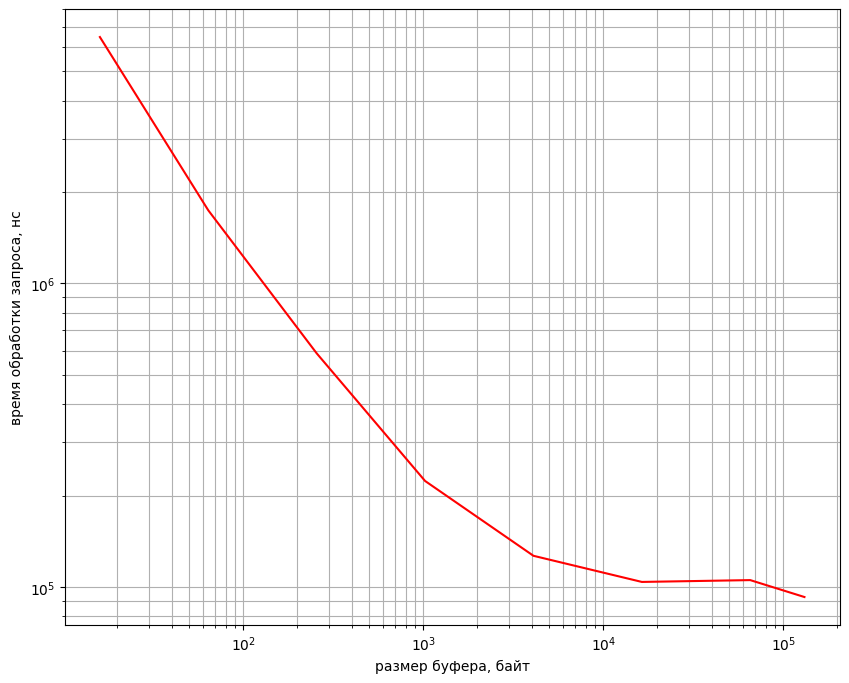
\includegraphics[width=\textwidth]{img/research.png}
    \caption{Зависимость времени обработки запроса от размера буфера}
    \label{fig:research}
\end{figure}
